\documentclass[a4paper,12pt,titlepage]{article}
\usepackage[T1]{fontenc}
\usepackage[brazil]{babel}
\usepackage[utf8x]{inputenc}
\usepackage{graphicx}
\usepackage{times}
\usepackage{ucs}
\usepackage{url}




\title{Trabalho de Conclusão de Curso \\ }


\author{Rodrigo L. M. Flores \and
        Orientador: Roberto Hirata Jr. }


\date{\today}

\begin{document}

\maketitle

\part{}

\section{Introdução}

O ponto de partida para este projeto é a necessidade de se fazer processamentos custosos de 
dados em bioinformática. Estes processamentos costumam ser combinatórios, o que os fazem
demorar um bom tempo para serem executados em um computador comum, sendo necessário utilizar recursos
computacionais de alta performance para obter os resultados em tempo hábil.

\subsection{Programação paralela e distribuída}

Uma abordagem clássica para se resolver esse problema é utilizar \textit{clusters} que são um grupo de computadores
ligados entre si de modo a parecer ser um único computador muito mais potente. \textit{Clusters} podem ser tanto máquinas
específicas para isso, produzidas com um alto custo e com um hardware específico para otimizar seu desempenho, ou 
pode ser utilizado o conceito de computação em grades: utilizar computadores pessoais, produzidos em massa e 
trabalhando em paralelo para fazer o processamento. 

O projeto \emph{Beowulf} é um dos exemplos de computação em grade: computadores pessoais baratos constituem uma grade dedicada 
que funciona como um super computador. De acordo com o projeto Beowulf, uma rede deste tipo provê o mesmo recurso computacional 
que um super computador custando de um terço a um décimo do preço. 

%Bibliografia projeto Beowulf


\subsection{Computação oportunista}
%Bibliografia Wikipedia


A computação voluntária é um tipo de computação distribuída no qual pessoas que possuem computadores podem doar processamento e
armazenamento ocioso de suas máquinas enquanto elas estiverem ociosas. Estes projetos normalmente têm um objetivo bem definide.

O primeiro projeto de Computação voluntária foi o \textit{Great Internet Mersenne Prime Search}, lançado em janeiro de 1996. 
Seu objetivo era encontrar números primos de Mersenne\footnote{Isto é, números primos na forma $M_n = 2^n - 1$}. Em seguida houveram 
muitos outros projetos e alguns utilizam um apelo social, de modo a obter mais doadores de processamento, um exemplo disso é o
o Folding At Home, que investiga o enrolamento de proteínas e que pode ajudar o desenvolvimentos de pesquisas contra 
Câncer, doença de Huntington, entre outras. 

Um dos projetos mais notáveis de computação voluntária foi o \textit{SETI@Home}. Os objetivos iniciais deste projeto eram: 

\begin{itemize}
  \item Provar a viabilidade e a praticidade de grades computacionais distribuídas;
  \item Fazer um trabalho útil e apoiar uma análise de observações para detectar vida inteligente fora da Terra.
\end{itemize}

Este projeto atraiu centenas de milhares de voluntários, porém só o primeiro objetivo teve sucesso: não foram encontrados sinais 
de vida inteligente fora da Terra. O middleware \emph{BOINC} foi um dos produtos obtidos deste projeto e hoje é utilizado em diversos
projetos. 

\subsection{Linguagens Interpretadas}

%Colocar bibliografia da wikipedia

Uma das possíveis divisões para linguagens de programação é se seus códigos são compilados ou simplismente interpretados. Enquanto no primeiro caso
é necessária a utilização de um programa para transformar o código fonte em código de máquina para ele poder então ser executado, mo segundo caso,
há a figura de um interpretador que não converte o programa para código de máquina, mas sim o interpreta e o executa. 

Linguagens interpretadas possuem vantagens e desvantagens: embora elas sejam mais fáceis de serem multiplataforma (basta o interpretador
estar disponível para aquela plataforma) e permitam escopo e tipagem dinâmica, também costumam ser menos eficientes que linguagens compiladas e 
a presença de um interpretador é obrigatória para sua execução. 

Dentre as linguagens interpretadas, uma que adquiriu destaque na área de estatística e bioinformática é a linguagem \emph{R}, que também 
pode ser utilizado como um ambiente. Esta linguagem já vem com as distribuições estatísticas mais usuais e possui uma extensibilidade 
poderosa, com bibliotecas que podem ser baixadas facilmente.


\subsection{Linguagens interpretadas e computação distribuída}

Embora já existam ótimas soluções para a execução distribuída de programas compilados como o
 MPI\footnote{disponível em \url{http://www.mcs.anl.gov/research/projects/mpi/}}, não se fala muito em soluções 
para execução distribuída de programas em linguagem interpretada. 
Para a linguagem \emph{R} há um pacote chamado \emph{gridR} que permite o uso do R com o \emph{Condor}, %Colocar note
um middleware para execução de programas em grades.  
Um outro trabalho que relaciona o R com computação distribuída é o \cite{Dias}: 
é utilizado o middleware baseado na tecnologia .NET \emph{Alchemi} e a interface \textit{COM}, junto com o pacote do 
\emph{RCom}.  


O artigo \cite{boinc} sobre a utilização do Middleware de computação voluntária BOINC como solução para computação 
em grade na Universidade de Extremadura na Espanha. Dentre os programas executados na grade, haviam
programas em R. Porém isso foi somente instalado em redes de computadores com computadores cujo sistema
operacional é o Linux. 

Seguindo este feito, este trabalho tem a intenção de construir algo semelhante nos laboratórios da rede CEC do IME/USP. Utilizando
não somente os computadores executando Linux, mas também os computadores cujo sistema operacional é o Microsoft Windows %Colocar marca registrada.
já que estes são uma parte considerável da rede.  

\section{Conceitos e tecnologias utilizadas}

O desenvolvimento do projeto incluiu diversas tecnologias, sendo as principais a linguagem de Programação \emph{R} e o middleware
para computação voluntária \emph{Boinc}.

\subsection{BOINC}

%Fonte wikipedia

O BOINC, cujo nome é uma sigla para \textit{Berkeley Open Infrastructure for Network Computing}, é um middleware 
para computação em grade e voluntária e foi criado na Universidade de Berkeley, Califórnia, Estados Unidos.

Inicialmente, o projeto consistia em gerenciar o projeto \textit{SETI@HOME} que possuía dois objetivos:

\begin{itemize}
	\item Provar a viabilidade e a praticidade do conceito ``computação em grade distribuída'';
	\item Fazer um trabalho científico útil fazendo uma análise observacional para detectar vida inteligente fora da Terra.
\end{itemize}

O primeiro objetivo foi concluído com sucesso e o resultado é o \textit{BOINC}. O segundo falhou: nenhuma evidência de 
vida inteligente fora da Terra foi encontrada. 

\subsubsection{Funcionamento do BOINC}

Cada unidade de processamento no Boinc é chamada de \emph{workunit} e é constítuida de arquivos executáveis e 
arquivos de entrada. Depois de processado, os arquivos de saída gerados são enviados para o servidor que
normalmente armazena estes arquivos em um banco de dados ou em um arquivo.

Para gerar um workunit são necessários dois arquivos XML, um deles detalhando a entrada e o 
outro detalhando a saída. Para facilitar a escrita do programa, precisamos escrever para cada arquivo um nome lógico 
que ao enviar e receber o cliente renomeia o arquivo. Por exemplo, temos um programa que lê um arquivo chamado 
\verb#input# e escreve no arquivo \verb#output#, para podermos ter muitos arquivos de entrada com nomes diferentes, quando
criamos uma \emph{workunit}, o servidor coloca um nome único e semelhante ao da workunit nos arquivos de entrada e saída que serão renomeados
pelo cliente para o nome lógico.

O processamento é realizado pelo cliente: o arquivo binário é executado e enquanto ele é executado há um checkpoint
que permite em caso de interrupções retomar o processamento de um determinado ponto. Finalizado o processamento, 
na próxima atualização o cliente avisará ao servidor que o processamento foi finalizado. Um diagrama do funcionamento pode
ser visto na figura \ref{funcionamento-boinc}. 


\begin{figure}[!h]
  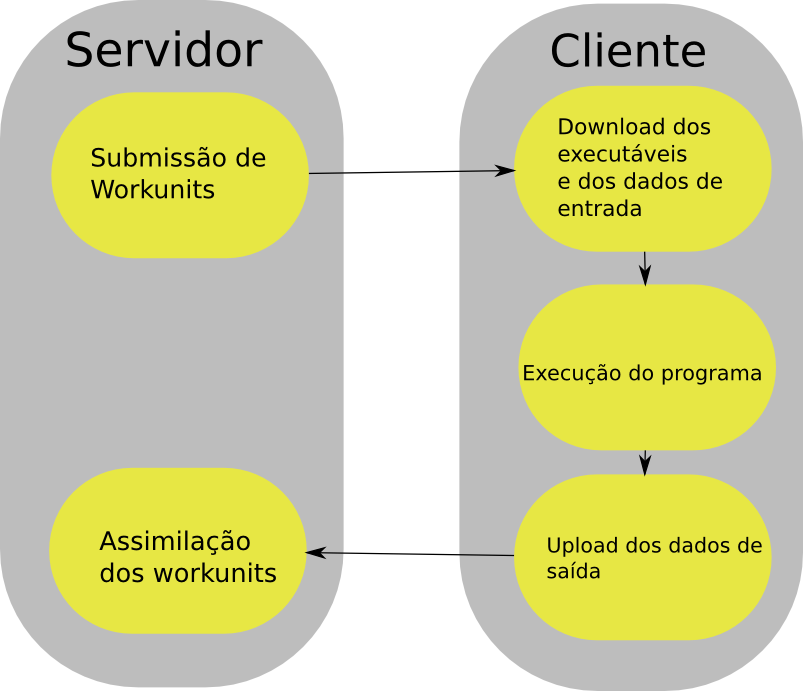
\includegraphics[scale=0.5]{boinc-schema.png}
  \caption{Funcionamento do Boinc}
  \label{funcionamento-boinc}
\end{figure}


\subsubsection{Wrapper}

%Fonte: página do Wrapper no site do BOINC

O \emph{Wrapper} é um programa escrito utilizando a \emph{api} do \emph{BOINC}, cujo objetivo é executar aplicações legadas, 
i.e. aplicações que não utilizam a API do \emph{BOINC}, utilizando o \textit{BOINC}. Há uma versão do Wrapper distribuída junto com o 
\textit{BOINC} que utiliza um arquivo XML, mas existe uma outra opção descrita no artigo %Artigo do Húngaro
que utiliza um shell para a execução dos aplicativos.

O arquivo XML de execução tem a seguinte estrutura:

\begin{verbatim}
<job_desc>
    <task>
        <application>foobar</application>
        [ <stdin_filename>stdin_file</stdin_filename> ]
        [ <stdout_filename>stdout_file</stdout_filename> ]
        [ <stderr_filename>stderr_file</stderr_filename> ]
        [ <command_line>--foo bar</command_line> ]
    </task>
    [ ... ]
</job_desc>
\end{verbatim}

Neste XML, o único campo obrigatório é o \emph{application}, que é a aplicação
que será executada e pode ser distribuída junto com a aplicação ou já existir no 
computador que o cliente estará instalado (para este segundo caso é necessário
informar o caminho inteiro do executável). É possível ter mais de uma tag
task, e o wrapper as executará sequencialmente. É de responsabilidade
do \textit{Wrapper} 

\subsection{R}

%Fonte wikipedia

A linguagem de programação estatística $R$ é uma implementação da linguagem $S$ e foi criada por John Ihaka e Robert
Gentleman na Universidade de Auckland, da Nova Zelândia. Hoje, a linguagem $R$ é uma linguagem considerada padrão
entre estatísticos no desenvolvimento de softwares estatísticos e na análise de dados. Há também um ambiente 
onde podemos utilizar a linguagem em um interpretador e gerar gráficos de alta qualidade. 

Por padrão, as distribuições estatísticas mais populares podem ser utilizadas e é muito mais simples que em 
linguagens como C, Java a manipulação de matrizes e tabelas de dados.Outro ponto importante na linguagem $R$ 
é a extensibilidade: é muito simples instalar bibliotecas. Hoje em dia, há
cerca de $2000$ bibliotecas no repositório principal (chamado de \emph{CRAN}, 
sigla de \textit{Comprehensible R Archive Network}) com as mais diversas funções 
(desde bibliotecas de gráficos específicos até métodos estatísticos mais complexos). 
Outro repositório bastante utilizado é o Bioconductor, que provê rotinas bastante utilizadas para o processamento
de dados da área de bioinformática.

\section{Atividades realizadas}

O início do projeto deu-se ainda em 2008, com a visita ao colégio Rainha da Paz na Lapa, onde o aluno de mestrado do \textit{IME}
Rodrigo Assirati Dias mantém uma grade de computadores com o middleware \textit{Alchemi} citada no trabalho %Artigo do Rodrigo
. Nesta visita foi possível esclarecer dúvidas, entender o funcionamento da grade e receber algumas dicas quanto à manutenção da grade. 
Após esse encontro, começou-se a buscar alternativas para o a computação de alta performance com o \textit{R}. Um primeiro pacote encontrado
que fazia esta função foi o \textit{GridR}, que permite submeter rotinas do \textit{R} para \textit{clusters}, máquinas remotas e 
grades. Um dos arcabouços possíveis para o uso deste pacote é o Condor %Colocar link 
, desenvolvido pela \textit{University of Wisconsin-Madison} e é bastante utilizado em empresas
de grande porte como a \textit{NASA} e pode ser executado tanto em sistemas
baseados em \textit{UNIX}, como em sistemas \textit{Windows}. Seguindo esta busca, encontramos o 
\textit{middleware} \textit{BOINC}, no artigo %Referência do BOINC
sendo utilizado para um propósito semelhante em um trabalho na Universidade de Extremadura, na Espanha 
e decidimos que a abordagem seria interessante para nosso trabalho.

Escolhido o \textit{middleware} nos focamos na instalação do servidor. A própria página do \textit{BOINC} 
possui um guia de instalação do servidor do \textit{middleware} no sistema \textit{Debian GNU\\Linux} e por
esta distribuição \textit{Linux} ser bastante conhecida por sua estabilidade, foi instalado este sistema no servidor.
Instalado o servidor, o foco foi em ter uma aplicação em R executando remotamente em uma grade de computadores. 
Este processo no sistema Linux foi relativamente simples: utilizando o ``truque do \textit{shebang}'' é possível 
colocar um script como executável e o \textit{wrapper} executá-lo como se fosse um arquivo compilado. Já para
o sistema Windows %Colocar marca registrada
o trabalho foi mais complicado: havia um bug nas configurações de compilação do \textit{wrapper} e até perceber isso
atrasou bastante o andamento do projeto. Passado isso, foi necessário utilizar um programa escrito em C, que apenas executava 
o interpretador junto com o arquivo com a rotina em \textit{R}.

Finalizado esta parte, nos focamos na aplicação a ser executada na grade. Para isso foi criado um programa em \textit{R} que
apenas acessava um arquivo e fazia alguns cálculos custosos. Isto foi então configurado para o mesmo programa poder
ser executado tanto em sistemas Windows como em sistemas Linux. Paralelamente a isso, foi pedido para a administração
da rede do \textit{CEC} para instalar o \textit{BOINC} nas máquinas da rede.

\section{Resultados e produtos obtidos}



\section{Conclusões}


\bibliographystyle{amsalpha}
\bibliography{bibliografia}


\newpage

\part{Parte subjetiva}

\section{Desafios e frustrações encontrados}

O curso de bacharelado em ciência da computação é um curso bastante denso e dificilmente temos tempo
para fazer todas as tarefas de todas as disciplinas. Então acredito que o meu maior desafio nestes anos de IME 
foi conciliar todas as tarefas e disciplinas, e infelizmente descartando alguma as vezes. 

\section{Disciplinas relevantes para o trabalho}

Diversas disciplinas foram relevantes para este trabalho:

\begin{itemize}
  \item \textbf{MAC110 - }
  \item \textbf{MAC122 - }
  \item \textbf{MAC211 - Laboratório de programação I} Ferramentas como versionamento de código, processamento de 
texto e o makefile foram essenciais para a elaboração deste trabalho de forma indireta e contribuiram com a 
boa qualidade do mesmo.
  \item \textbf{MAC242 - Laboratório de programação II} Linguagens de script facilitam bastante o trabalho de tarefas 
repetitivas e o boa parte do que sei sobre este tipo de linguagem eu aprendi neste curso.
  \item \textbf{MAC338 - Análise de algoritmos} Este curso contribuiu indiretamente com minha formação como cientista da computação i
e muitos dos conceitos aprendidos neste curso ajudaram o entendimento melhor de algoritmos e soluções.
  \item \textbf{Programação paralela e distribuída}
  \item \textbf{MAC422 - Sistemas Operacionais} Saber como um programa é executado, como o sistema gerencia essas execução e como a tabela de processos
funciona é essencial quando se trabalha com uma grade de computadores.  
\end{itemize}

% desafios e frustrações encontrados;
% lista das disciplinas cursadas no BCC mais relevantes para o trabalho;
% observações sobre a aplicação de conceitos estudados nas disciplinas do curso;
% se o aluno fosse continuar atuando na área em que realizou o trabalho, que passos tomaria para aprimorar os conhecimentos relevantes para esta atividade?
\end{document}
